\documentclass{vkr}
\usepackage[english, russian]{babel} % переносы
\usepackage{graphicx} % для вставки картинок
\graphicspath{{images/}} % путь к изображениям
\usepackage[hidelinks]{hyperref}
\usepackage{float} % определяет метод H для рисунка с переносом на следующую страницу, ели не помещается
\usepackage{pdflscape}
\addto{\captionsrussian}{\renewcommand{\refname}{СПИСОК ИСПОЛЬЗОВАННЫХ ИСТОЧНИКОВ}}
\usepackage{xltabular} % для вставки таблиц
\usepackage{makecell}
\renewcommand\theadfont{} % шрифт в /thead
\usepackage{array} % для определения новых типов столбцов таблиц
\newcolumntype{T}{>{\centering\arraybackslash}X} % новый тип столбца T - автоматическая ширина столбца с выравниванием по центру
\newcolumntype{R}{>{\raggedleft\arraybackslash}X} % новый тип столбца R - автоматическая ширина столбца с выравниванием по правому краю
\newcolumntype{C}[1]{>{\centering\let\newline\\\arraybackslash\hspace{0pt}}m{#1}} % новый тип столбца C - фиксированная ширина столбца с выравниванием по центру
\newcolumntype{r}[1]{>{\raggedleft\arraybackslash}p{#1}} % новый тип столбца r - фиксированная ширина столбца с выравниванием по правому краю
\newcommand{\centrow}{\centering\arraybackslash} % командой \centrow можно центрировать одну ячейку (заголовок) в столбце типа X или p, оставив в оcтальных ячейках другой тип выравнивания
\newcommand{\finishhead}{\endhead\hline\endlastfoot}
\newcommand{\continuecaption}[1]{\caption*{#1}\\ \hline }
\usepackage{etoolbox}
\AtBeginEnvironment{xltabular}{\refstepcounter{tablecnt}} % подсчет таблиц xltabular, обычные таблицы подсчитываются в классе

\usepackage[tableposition=top]{caption} % подпись таблицы вверху
\captionsetup{strut=off}
\setlength{\intextsep}{0pt} % Vertical space above & below [h] floats
\setlength{\textfloatsep}{0pt} % Vertical space below (above) [t] ([b]) floats
\DeclareCaptionLabelFormat{gostfigure}{Рисунок #2} %подпись рисунка
\DeclareCaptionLabelFormat{gosttable}{Таблица #2} %подпись таблицы
\DeclareCaptionLabelSeparator{gost}{~--~} %разделитель в рисунках и таблицах
\captionsetup{labelsep=gost}
\captionsetup[figure]{aboveskip=10pt,belowskip=4mm,justification=centering,labelformat=gostfigure} % настройка подписи рисунка
\captionsetup[table]{font={stretch=1.41},skip=0pt,belowskip=0pt,aboveskip=8.5pt,singlelinecheck=off,labelformat=gosttable} % настройка подписи таблицы

\setlength{\LTpre}{8mm} % отступ сверху таблицы
\setlength{\LTpost}{6mm} % отступ снизу таблицы

\usepackage{enumitem}
\setlist{nolistsep,wide=\parindent,itemindent=*} % отступы вокруг списков, выравнивание с учетом разделителя

\usepackage{color} %% это для отображения цвета в коде
\usepackage{listings} %% листинги кода
\setmonofont[Scale=0.7]{Verdana} % моноширный шрифт для листинга

\definecolor{codegreen}{rgb}{0,0.6,0}
\definecolor{codegray}{rgb}{0.5,0.5,0.5}
\definecolor{codepurple}{rgb}{0.58,0,0.82}

\lstset{ %
language=C,                 % выбор языка для подсветки (здесь это С)
numbers=left,               % где поставить нумерацию строк (слева\справа)
numberstyle=\tiny,           % размер шрифта для номеров строк
stepnumber=1,                   % размер шага между двумя номерами строк
numbersep=5pt,                % как далеко отстоят номера строк от подсвечиваемого кода
commentstyle=\color{codegreen},
keywordstyle=\color{magenta},
numberstyle=\tiny\color{codegray},
stringstyle=\color{codepurple},
basicstyle=\linespread{0.95}\ttfamily,
backgroundcolor=\color{white}, % цвет фона подсветки - используем \usepackage{color}
showspaces=false,            % показывать или нет пробелы специальными отступами
showstringspaces=false,      % показывать или нет пробелы в строках
showtabs=false,             % показывать или нет табуляцию в строках
frame=single,              % рисовать рамку вокруг кода
tabsize=2,                 % размер табуляции по умолчанию равен 2 пробелам
captionpos=t,              % позиция заголовка вверху [t] или внизу [b] 
breaklines=true,           % автоматически переносить строки (да\нет)
breakatwhitespace=false, % переносить строки только если есть пробел
escapeinside={\%*}{*)}   % если нужно добавить комментарии в коде
}

\makeatletter % чтобы допускались русские комментарии в листингах
\lst@InputCatcodes
\def\lst@DefEC{%
 \lst@CCECUse \lst@ProcessLetter
  ^^80^^81^^82^^83^^84^^85^^86^^87^^88^^89^^8a^^8b^^8c^^8d^^8e^^8f%
  ^^90^^91^^92^^93^^94^^95^^96^^97^^98^^99^^9a^^9b^^9c^^9d^^9e^^9f%
  ^^a0^^a1^^a2^^a3^^a4^^a5^^a6^^a7^^a8^^a9^^aa^^ab^^ac^^ad^^ae^^af%
  ^^b0^^b1^^b2^^b3^^b4^^b5^^b6^^b7^^b8^^b9^^ba^^bb^^bc^^bd^^be^^bf%
  ^^c0^^c1^^c2^^c3^^c4^^c5^^c6^^c7^^c8^^c9^^ca^^cb^^cc^^cd^^ce^^cf%
  ^^d0^^d1^^d2^^d3^^d4^^d5^^d6^^d7^^d8^^d9^^da^^db^^dc^^dd^^de^^df%
  ^^e0^^e1^^e2^^e3^^e4^^e5^^e6^^e7^^e8^^e9^^ea^^eb^^ec^^ed^^ee^^ef%
  ^^f0^^f1^^f2^^f3^^f4^^f5^^f6^^f7^^f8^^f9^^fa^^fb^^fc^^fd^^fe^^ff%
  ^^^^20ac^^^^0153^^^^0152%
  % Basic Cyrillic alphabet coverage
  ^^^^0410^^^^0411^^^^0412^^^^0413^^^^0414^^^^0415^^^^0416^^^^0417%
  ^^^^0418^^^^0419^^^^041a^^^^041b^^^^041c^^^^041d^^^^041e^^^^041f%
  ^^^^0420^^^^0421^^^^0422^^^^0423^^^^0424^^^^0425^^^^0426^^^^0427%
  ^^^^0428^^^^0429^^^^042a^^^^042b^^^^042c^^^^042d^^^^042e^^^^042f%
  ^^^^0430^^^^0431^^^^0432^^^^0433^^^^0434^^^^0435^^^^0436^^^^0437%
  ^^^^0438^^^^0439^^^^043a^^^^043b^^^^043c^^^^043d^^^^043e^^^^043f%
  ^^^^0440^^^^0441^^^^0442^^^^0443^^^^0444^^^^0445^^^^0446^^^^0447%
  ^^^^0448^^^^0449^^^^044a^^^^044b^^^^044c^^^^044d^^^^044e^^^^044f%
  ^^^^0401^^^^0451%
  %%%
  ^^00}
\lst@RestoreCatcodes
\makeatother


% Режим шаблона (должен быть включен один из трех)
%\ВКРtrue
\Практикаtrue
%\Курсоваяtrue

%\newcommand{\Дисциплина}{<<Проектирование и архитектура программных систем>>} % для курсовой
%\newcommand{\КодСпециальности}{09.03.04} % Курсовая
%\newcommand{\Специальность}{Программная инженерия} % Курсовая
%\newcommand{\Тема}{Разработка web-сайта «Русатом – Аддитивные технологии» на платформе} % ВКР Курсовая
\newcommand{\ТемаВтораяСтрока}{Программное обеспечение для управления работой центра здорового питания}
\newcommand{\ГдеПроводитсяПрактика}{ООО «МЦОБ. Онлайн-сервисы»} % для практики
\newcommand{\РуководительПрактПредпр}{Куркина А. В.} % для практики
\newcommand{\ДолжнРуководительПрактПредпр}{директор} % для практики
\newcommand{\РуководительПрактУнивер}{Чаплыгин А. А.} % для практики
\newcommand{\ДолжнРуководительПрактУнивер}{к.т.н. доцент} % для практики
\newcommand{\Автор}{Ю. С. Коротаева}
\newcommand{\АвторРод}{Коротаевой Ю.С.}
\newcommand{\АвторПолностьюРод}{Коротаевой Юлии Сергеевны} % для практики
\newcommand{\Шифр}{19-06-0305}
\newcommand{\Курс}{5 } % для практики
\newcommand{\Группа}{ПО-91з}
%\newcommand{\Руководитель}{А. А. Чаплыгин} % для ВКР и курсовой
%\newcommand{\Нормоконтроль}{А. А. Чаплыгин} % для ВКР
%\newcommand{\ЗавКаф}{А. В. Малышев} % для ВКР
%\newcommand{\ДатаПриказа}{«07» апреля 2023~г.} % для ВКР
%\newcommand{\НомерПриказа}{1505-с} % для ВКР
%\newcommand{\СрокПредоставления}{«13» июня 2023~г.} % для ВКР, курсового

\begin{document}
\maketitle
\ifПрактика{}\else{
   \newpage
\begin{center}
\large\textbf{Минобрнауки России}

\large\textbf{Юго-Западный государственный университет}
\vskip 1em
\normalsize{Кафедра программной инженерии}
\vskip 1em
\ifВКР{
        \begin{flushright}
        \begin{tabular}{p{.4\textwidth}}
        \centrow УТВЕРЖДАЮ: \\
        \centrow Заведующий кафедрой \\
        \hrulefill \\
        \setarstrut{\footnotesize}
        \centrow\footnotesize{(подпись, инициалы, фамилия)}\\
        \restorearstrut
        «\underline{\hspace{1cm}}»
        \underline{\hspace{3cm}}
        20\underline{\hspace{1cm}} г.\\
        \end{tabular}
        \end{flushright}
        }\fi
\end{center}
\vspace{1em}
  \begin{center}
  \large
\ifВКР{
ЗАДАНИЕ НА ВЫПУСКНУЮ КВАЛИФИКАЦИОННУЮ РАБОТУ
  ПО ПРОГРАММЕ БАКАЛАВРИАТА}
  \else
ЗАДАНИЕ НА КУРСОВУЮ РАБОТУ (ПРОЕКТ)
\fi
\normalsize
  \end{center}
\vspace{1em}
{\parindent0pt
  Студента \АвторРод, шифр\ \Шифр, группа \Группа
  
1. Тема «\Тема\ \ТемаВтораяСтрока»
\ifВКР{
утверждена приказом ректора ЮЗГУ от \ДатаПриказа\ № \НомерПриказа
}\fi.

2. Срок предоставления работы к защите \СрокПредоставления

3. Исходные данные для создания программной системы:

3.1. Перечень решаемых задач:}

\renewcommand\labelenumi{\theenumi)}

\begin{enumerate}
\item проанализировать IT-инфраструктуру предприятия;
\item  разработать концептуальную модель системы управления IT-ин\-фра\-струк\-турой предприятия на основе подхода к управлению и организации ИТ-услуг ITSM;
\item спроектировать программную систему управления IT-ин\-фра\-струк\-турой предприятия;
\item сконструировать и протестировать программную систему управления IT-инфраструктурой предприятия.
\end{enumerate}

{\parindent0pt
  3.2. Входные данные и требуемые результаты для программы:}

\begin{enumerate}
\item Входными данными для программной системы являются: данные
справочников комплектующих, конфигураций, ПО, критериев качества SLA,
ИТ-услуг, департаментов компании; технические данные ИТ-ресурсов; данные входящих заявок на ИТ-ресурсы; данные запросов поставщикам на комплектующие.
\item Выходными данными для программной системы являются: сформированные заявки на обслуживание ИТ-ресурсов; сформированные запросы на
закупку комплектующих; сведения о выполненных работах по заявкам; статусы заявок; выходные отчеты (инфографика) – по качеству услуг, по состоянию ИТ-ресурсов, по деятельности ИТ-отдела, по стоимости обслуживания
ИТ-ресурсов, воронка заявок.
\end{enumerate}

{\parindent0pt

  4. Содержание работы (по разделам):
  
  4.1. Введение
  
  4.1. Анализ предметной области
  
4.2. Техническое задание: основание для разработки, назначение разработки,
требования к программной системе, требования к оформлению документации.

4.3. Технический проект: общие сведения о программной системе, проект
данных программной системы, проектирование архитектуры программной системы, проектирование пользовательского интерфейса программной системы.

4.4. Рабочий проект: спецификация компонентов и классов программной системы, тестирование программной системы, сборка компонентов программной системы.

4.5. Заключение

4.6. Список использованных источников

5. Перечень графического материала:

\списокПлакатов

\vskip 2em
\begin{tabular}{p{6.8cm}C{3.8cm}C{4.8cm}}
Руководитель \ifВКР{ВКР}\else работы (проекта) \fi & \lhrulefill{\fill} & \fillcenter\Руководитель\\
\setarstrut{\footnotesize}
& \footnotesize{(подпись, дата)} & \footnotesize{(инициалы, фамилия)}\\
\restorearstrut
Задание принял к исполнению & \lhrulefill{\fill} & \fillcenter\Автор\\
\setarstrut{\footnotesize}
& \footnotesize{(подпись, дата)} & \footnotesize{(инициалы, фамилия)}\\
\restorearstrut
\end{tabular}
}

\renewcommand\labelenumi{\theenumi.}

   \abstract{РЕФЕРАТ}

Объем работы равен \formbytotal{lastpage}{страниц}{е}{ам}{ам}. Работа содержит \formbytotal{figurecnt}{иллюстраци}{ю}{и}{й}, \formbytotal{tablecnt}{таблиц}{у}{ы}{}, \arabic{bibcount} библиографических источников и \formbytotal{числоПлакатов}{лист}{}{а}{ов} графического материала. Количество приложений – 2. Графический материал представлен в приложении А. Фрагменты исходного кода представлены в приложении Б.

Перечень ключевых слов: Система, диета, врач, врач-диетолог, КБЖУ, болезнь, продукты, карта пациента, поиск, услуги, сервер, информационные технологии, веб-форма, компоненты, база данных, подсистема, информационный блок, администратор, пользователь, web-сайт, JavaScript, React, SQLite.

Объектом разработки является web-сайт для работы центра здорового питания.

Целью выпускной квалификационной работы является разработка web-сайта для упрощения ведения записей о пациенте  врачу-диетологу в центре здорового питания.

В процессе создания web-сайта были выделены основные сущности обеспечивающие работу с сущностями предметной области, а также корректную работу web-сайта, разработаны разделы, содержащие информацию о пациентах, Врачах, продуктах и болезнях.

При создании клиент-серверного приложения применялись технологии событийно-ориентированного программирования, современные средства разработки веб-приложения.

Для размещения программной системы компьютер должен обладать следующими характеристиками: процессор с тактовой частотой 2.4 ГГц, ОЗУ 1 Гб, место на жестком диске не менее 2 Гб, операционная система Windows 10, версией не ниже 2004, либо операционная система Linux с версией ядра не менее 4.х, установленное на компьютер средство контейнеризации Docker. 
Разработанный программный продукт находится на стадии предложения внедрения.

\selectlanguage{english}
\abstract{ABSTRACT}
  
The volume of work is \formbytotal{lastpage}{page}{}{s}{s}. The work contains \formbytotal{figurecnt}{illustration}{}{s}{s}, \formbytotal{tablecnt}{table}{}{s}{s}, \arabic{bibcount} bibliographic sources and \formbytotal{числоПлакатов}{sheet}{}{s}{s} of graphic material. The number of applications is 2. The graphic material is presented in annex A. The layout of the site, including the connection of components, is presented in annex B.

List of keyword users: System, diet, doctor, dietician, KBZHU, disease, products, patient card, search, services, server, information technology, web form, components, database, subsystem, information block, administrator, web -website, JavaScript, React, SQLite.

The object of development is a website for a healthy nutrition center.

The purpose of the final qualifying work is to develop a website to simplify the maintenance of healthy eating records for a dietitian patient.

In the process of creating the website, the basic principles of ensuring work with the essence of the subject area, as well as the correct operation of the website, were highlighted, sections containing information about patients, doctors, products and diseases were developed.

When creating a client-server application, event-oriented programming technologies and modern web application development tools are used.

To host a computer software system, the following conditions must be met: a processor with a clock frequency of 2.4 GHz, RAM 1 GB, hard disk space of at least 2 GB, the Windows 10 operating system, rating not lower than 2004, or the Linux operating system with a flagship kernel not less than 4..x, Docker containerization tool installed on the computer.
The developed software product is at the stage of offering software.
\selectlanguage{russian}
}\fi
\tableofcontents
\section*{ОБОЗНАЧЕНИЯ И СОКРАЩЕНИЯ}

БД -- база данных.

ИС -- информационная система.

ИТ -- информационные технологии. 

ОМТС -- отдел материально-технического снабжения. 

ПО -- программное обеспечение.

РП -- рабочий проект.

СУБД -- система управления базами данных.

ТЗ -- техническое задание.

ТП -- технический проект.

HTML (HyperText Markup Language) -- стандартизированный язык гипертекстовой разметки документов для просмотра веб-страниц в браузере.

КБЖУ -- белки, жиры и углеводы в рамках суточной калорийности.

\ifПрактика{}\else{\section*{ВВЕДЕНИЕ}
\addcontentsline{toc}{section}{ВВЕДЕНИЕ}
Актуальность темы. На данный момент в нашей стране не существует программного обеспечения для врачей-диетологов. Есть программа для записи пациента на прием, отдельный сайт со стандартными диетами, которые назначают по установленному заболеванию желудочно-кишечного тракта у клиента, так же отдельно можно найти калькулятор калорий. Одного ПО по всем этим пунктам нет, поэтому и было принято решение, помочь центрам здорового питания для упрощения их работы.

\emph{Цель настоящей работы} – разработка web-сайта компании для привлечения новой аудитории, увеличения заказов, рекламы продукции и услуг компании. Для достижения поставленной цели необходимо решить \emph{следующие задачи:}
\begin{itemize}
\item провести анализ предметной области;
\item разработать концептуальную модель web-сайта;
\item спроектировать web-сайт;
\item реализовать сайт средствами web-технологий.
\end{itemize}

\emph{Структура и объем работы.} Отчет состоит из введения, 4 разделов основной части, заключения, списка использованных источников, 2 приложений. Текст выпускной квалификационной работы равен \formbytotal{page}{страниц}{е}{ам}{ам}.

\emph{Во введении} сформулирована цель работы, поставлены задачи разработки, описана структура работы, приведено краткое содержание каждого из разделов.

\emph{В первом разделе} на стадии описания технической характеристики предметной области приводится сбор информации о деятельности компании, для которой осуществляется разработка сайта.

\emph{Во втором разделе} на стадии технического задания приводятся требования к разрабатываемому сайту.

\emph{В третьем разделе} на стадии технического проектирования представлены проектные решения для web-сайта.

\emph{В четвертом разделе} приводится список классов и их методов, использованных при разработке сайта, производится тестирование разработанного сайта.

В заключении излагаются основные результаты работы, полученные в ходе разработки.

В приложении А представлен графический материал.
В приложении Б представлены фрагменты исходного кода. 
}\fi
\section{Анализ предметной области}
\subsection{Актуальность цифровизации медицины в наше время}

Актуальность темы. На данный момент в нашей стране не существует программного обеспечения для врачей-диетологов. Есть программа для записи пациента на прием, отдельный сайт со стандартными диетами, которые назначают по установленному заболеванию желудочно-кишечного тракта у клиента, так же отдельно можно найти калькулятор калорий. Одного ПО по всем этим пунктам нет, поэтому было принято решение, помочь центрам здорового питания в упрощении их работы, создав веб-сайт, где совмещены все необходимые функции для работы врачей-диетолог с пациентами.

Цифровизация медицины – это процесс внедрения и применения ИТ-технологий, цифровых сервисов в отрасли, которая затрагивает все процессы – от управления системой здравоохранения до практической деятельности врачей на местах. Цифровизация предполагает качественную трансформацию медицины, повышение ее эффективности за счет оптимизации и автоматизации системы, организации четкой работы всех ее звеньев как в государственном, так и частном сегменте.

В наши дни система здравоохранения сталкивается с ежедневными вызовами, требующими от нее проактивных решений. Цифровизация медицины в России, начавшаяся десятилетия назад и на сегодняшний день набравшая высокие обороты, – логичный ответ на воздействующие внешние факторы. Можно сказать, что процесс оптимизации, качественной трансформации отрасли набрал динамику и стал одним из центральных буквально за последние несколько лет. Пережитые годы пандемии и в разы возросшая нагрузка на систему оказания медицинской помощи населению, потребовавшая оперативного внедрения современных ИТ-решений в лечебные процессы, всеобщая тенденция на цифровизацию жизни, использование гаджетов, в том числе в вопросах заботы о здоровье, разработка и распространение многочисленных онлайн приложений и сервисов, телемедицинские консультации, развитие систем искусственного интеллекта – все это происходит здесь и сейчас, на наших глазах внедряются инновационные технологии в медицине, что оказывает колоссальное влияние на качественную трансформацию отрасли и как следствие на совершенствование лечебного процесса, качество обслуживания пациентов, а также управление системой в целом.


\subsection{Цифровизация в медицине и здравоохранении: задачи и вызовы}

В конце 2021 года Правительство Российской Федерации определило стратегию развития системы (цифровизация в медицине и здравоохранении) на ближайшие несколько лет, выделив основные направления в области цифровой трансформации. Во-первых, это создание в здравоохранении единого цифрового контура на основе ЕГИСЗ, а также разработка и внедрение на федеральном уровне медицинских платформенных решений.

Благодаря реализации данных стратегических инициатив будет решен ряд стоящих перед отраслью задач:

\begin{enumerate}
	\item Обеспечение взаимодействия различных медицинских учреждений между собой и государственными системами.
	\item Станет возможным дистанционный лицензионный контроль медицинской деятельности.
	\item Обеспечение внедрения системы электронных рецептов на всей территории страны.
	\item Внедрение системы контроля полноты выполнения клинических рекомендаций на всех этапах лечебного процесса.
\end{enumerate}

Кроме того, современные технологии в медицине позволят оптимизировать процессы управления системой здравоохранения в целом, учитывать первичные медицинские данные, активно использовать структурированные электронные медицинские документы, а также осуществить постепенный переход на электронный документооборот в отрасли.

Цифровизация медицины, по мнению экспертов, должна способствовать следующим аспектам:

\begin{enumerate}
	\item Существенно минимизировать затраты на работу системы.
	\item Значительно повысить качество оказываемых медицинских услуг.
	\item Обеспечить более широкую доступность медицинской помощи.
	\item Оптимизировать время, которое тратит пациент на получение услуг (к примеру, ускорение процесса через внедрение сервиса записи на прием к специалисту).
	\item Сократить время работы самого врача (внедрение систем поддержки принятий решений, ведение электронной карты с ее быстрым заполнением через систему преобразования голоса в текст).
\end{enumerate}

Процесс цифровизации системы здравоохранения в нашей стране стартовал еще в 2011 году, именно в это время было сформулировано понятие «Цифровой контур здравоохранения». Конечно, не все намеченные задачи до сих пор удалось превратить в жизнь. Однако, отрицать существенный прогресс в этом процессе также бессмысленно. Получившие повсеместное распространение электронные больничные листы, внедрение электронных справок, свидетельств о рождении и смерти. Мгновенная отправка и обмен оцифрованными рентгеновскими снимками, которые позволили ставить рентгенологу точный диагноз удаленно, что обеспечило возможность создания в период эпидемии коронавируса специализированных центров, диагностирующих пациентов с патологиями на всей территории РФ, развитие системы искусственного интеллекта, системы маршрутизации пациентов, создание порталов для врачей и пациентов, содержащие полные и достоверные сведения о здоровье, пройденных процедурах, анализах, диагнозах. Все это, безусловно, уже сегодня качественно меняет существующую систему.
Кроме того, не так давно Министерство экономического развития инициировало эксперимент по дистанционной торговле рецептурными лекарствами, опубликовав законопроект с соответствующими поправками к существующему законодательству. Так в рамках экспериментального правового режима можно будет дистанционно получать и отоваривать рецепты на такие препараты, как антибиотики, лекарства для лечения хронических заболеваний сердца, бронхиальной астмы, диабета, и другие.

\subsection{Обоснование выбора технологии проектирования}

На сегодняшний день информационный рынок, поставляющий программные решения в выбранной сфере, предлагает множество продуктов, позволяющих достигнуть поставленной цели – разработки web-сайта.

\subsubsection{Описание используемых технологий и языков программирования}

В процессе разработки web-сайта используются программные средства и языки программирования TypeScript, SQL. Каждое программное средство и каждый язык программирования применяется для круга задач, при решении которых они необходимы.

\subsubsection{JavaScript-библиотека -- React}

React — это JavaScript-библиотека для создания пользовательских интерфейсов. Обратите внимание, что это именно библиотека, а не фреймворк. React часто называют фреймворком, но это ошибка. Во-первых, его использование ни к чему вас не обязывает, не формирует «фрейм» проекта. Во-вторых, React выполняет единственную задачу: показывает на странице компонент интерфейса, синхронизируя его с данными приложения, и только этой библиотеки в общем случае недостаточно для того, чтобы полностью реализовать проект.

Вскоре после появления React и подобные ему решения (Vue.js, Svelte) практически захватили мир фронтенда: потому что они помогают решать проблемы, основываясь на идее декларативного программирования, а не на императивном подходе.

— Декларативный подход состоит в описании конечного результата (что мы хотим получить).

— При императивном подходе описываются конкретные шаги для достижения конечного результата (как мы хотим что-то получить).

Оказалось, что декларативный подход отлично подходит для создания интерфейсов, и он прижился в сообществе. Этот подход работает не только в вебе: сравнительно недавно компания Apple представила фреймворк SwiftUI, основанный на тех же принципах.


\subsubsection{Язык программирования JavaScript}

\paragraph{Достоинства языка JavaScript}

JavaScript – объектно-ориентированный язык программирования для написания сценариев \cite{javascript}. Чаще всего JavaScript используется для написания сценариев работы с web-страницами, отображаемыми web-браузером. Web-бра\-у\-зер интерпретирует код сценария языка JavaScript, и на основе описанных в сценарии действий производит манипуляции с разметкой web-страницы. Посредством языка JavaScript реализуется возможность программирования на стороне клиента. Предоставляет возможность доступа к элементам разметки web-страницы посредством объектов. При создании сценариев на языке JavaScript приходится сталкиваться с трудностями, связанными с тем, что различные web-браузеры могут по-разному интерпретировать эти сценарии. Серьезные трудности возникают, если какой-либо из браузеров не поддерживает тот или иной объект, метод или свойство. Наиболее практичным способом решения данной проблемы является использование библиотеки jQuery. Данная библиотека реализована на языке JavaScript и расширяет возможности данного языка, нивелируя различия между браузерами.

\paragraph{Недостатки языка Javascript}
\begin{enumerate}
	\item Язык компилируется в момент исполнения кода. Каждый раз, когда вы открываете сайт, javascript код начинает компилироваться. Как минимум увеличивается время выполнения программы.
	\item Отсутствует типизация данных. Проблема всех скриптовых языков. Пока выполнение кода не дойдет до нужной строчки, не узнаешь работает ли она. А ведь значительную часть по поиску ошибок мог бы взять на себя компилятор, если бы знал типы данных, с которыми он работает. Да и по скорости выполнения, типизированный код быстрее.
	\item Не привычная для многих программистов объектная модель. Классы и наследование классов присутствует, но оно сильно отличается от привычной многим реализаций в языках программирования C++ Java.
\end{enumerate}
\section{Техническое задание}
\subsection{Основание для разработки}

Основанием для разработки информационно-вычислительной системы является задание на выпускную квалификационную работу по программе бакалавра «Программное обеспечение для управления работой центра здорового питания» согласно приказу №5197-с от 13.11.2023. «Об утверждении тем выпускных квалификационных работ и руководителей выпускных квалификационных работ».

Необходимо спроектировать и разработать сайт, который должен способствовать упрощению работы для врачей-диетологов в центре здорового питания.

Интернет-сайт представляет собой набор взаимосвязанных электронных страниц, которые сгруппированы по разделам, содержащие текстовую, графическую. Сайт располагается в Интернете по определенному адресу – доменному имени сайта в виде www.имя\_сайта.ru. Каждая страница web-сайта – это текстовый документ, написанный на языке программирования (HTML, CSS, JavaScript и т.д.).

\subsection{Цель и назначение разработки}

Программный продукт предназначен для компаний связанных со здоровым питанием, чтобы упростить рабочий процесс.Данный программный продукт предназначен для использования в различного рода коммерческих и бюджетных организациях.

Задачами данной разработки являются:
\begin{itemize}
\item создание разделов сайта;
\item реализация формы для входа;
\item реализация формы для регистрации пациента;
\item реализация формы карты пациента;
\item реализация формы для назначения диеты;
\item реализация калькулятора подсчета КБЖУ;
\item создание удобного поиска по сайту.
\end{itemize}

\subsection{Требования пользователя к интерфейсу web-сайта}

Сайт должен включать в себя:
\begin{itemize}
    \item авторизацию;
    \item навигацию по разделам;
    \item регистрация пациента;
    \item просмотр списка пациентов;
    \item просмотр карты пациента;
    \item просмотр списка продуктов с пищевой ценностью;
    \item просмотр списка болезней желудочно-кишечного тракта.
\end{itemize}

Для взаимодействия с системой должен быть разработан интерфейс по макетам представленных на рисунках.

Макет страницы "Авторизация" представлен на рисунке ~\ref{fig:image}.
\begin{figure}[th]
	\centering
	
\includegraphics[width=1\linewidth]{images/Авторизация}
	\caption{Макет страницы "Авторизация"}
	\label{fig:image}
\end{figure}

Макет страницы навигационной панели представлена на рисунке ~\ref{fig:imagen}.
\begin{figure}[H]
	\centering
	
\includegraphics[width=1\linewidth]{images/Нав.панель}
	\caption{Навигационная панель}
	\label{fig:imagen}
\end{figure}

Макет страницы регистрация пациента представлена на рисунке ~\ref{fig:imagep}.
\begin{figure}[H]
	\centering
	\includegraphics[width=1\linewidth]{"images/Регистрация пациента"}
	\caption{Регистрация пациента}
	\label{fig:imagep}
\end{figure}

Макет страницы список пациентов представлена на рисунке ~\ref{fig:images}.
\begin{figure}[H]
	\centering
	\includegraphics[width=1\linewidth]{"images/Список пациентов"}
	\caption{Список пациентов}
	\label{fig:images}
\end{figure}

Макет страницы информация о пациенте представлена на рисунке ~\ref{fig:imagein}.
\begin{figure}[H]
	\centering
	\includegraphics[width=1\linewidth]{"images/Инфа о пациенте"}
	\caption{Список пациентов}
	\label{fig:imagein}
\end{figure}

Макет страницы списка продуктов представлена на рисунке ~\ref{fig:imagepr}.
\begin{figure}[H]
	\centering
	\includegraphics[width=1\linewidth]{"images/Список продуктов"}
	\caption{Список продуктов}
	\label{fig:imagepr}
\end{figure}

Макет страницы списка болезней представлена на рисунке ~\ref{fig:imagebl}.
\begin{figure}[H]
	\centering
	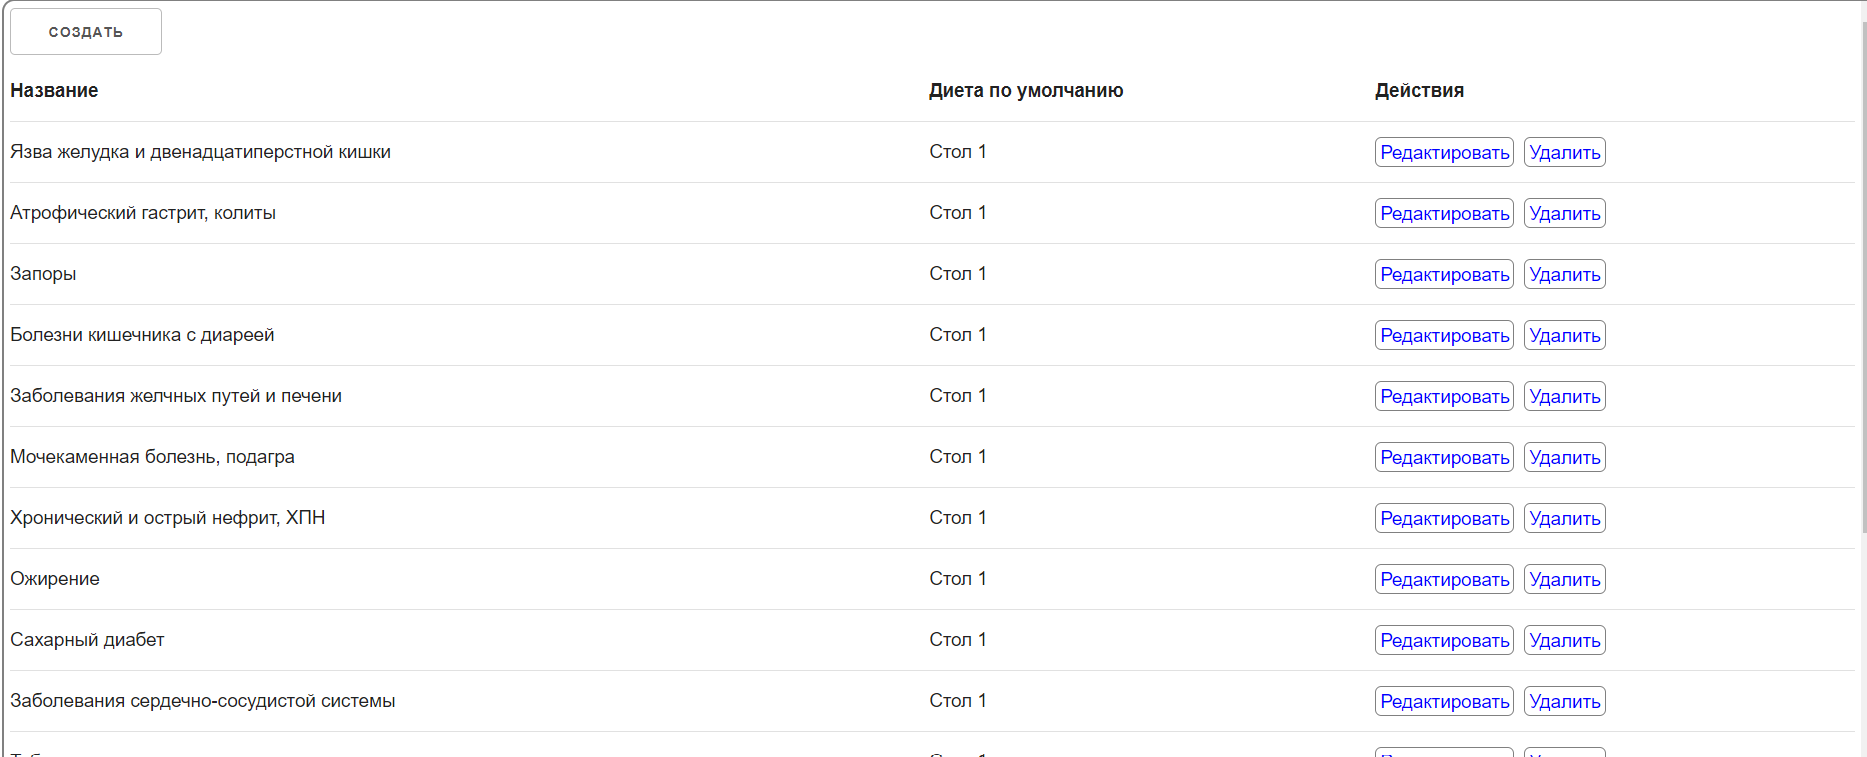
\includegraphics[width=1\linewidth]{images/Болезни}
	\caption{Список болезней}
	\label{fig:imagebl}
\end{figure}

%\vspace{-\figureaboveskip} % двойной отступ не нужен (можно использовать, если раздел заканчивается картинкой)

\subsection{Функциональные требования к программной системе}

Разрабатываемая система должна иметь несколько ролей
пользователей:

\begin{itemize}
	\item администратор;
	\item врач.
\end{itemize}

Для администратора должны быть предусмотрены следующие функции в разрабатываемой системе: 

\begin{itemize}
	\item авторизация;
	\item просмотр списка врачей;
	\item создание пользователя;
	\item редактирование пользователя;
	\item удаление пользователя;
	\item просмотр списка продуктов;
	\item добавление продукта;
	\item редактирование продукта;
	\item удаление продукта;
	\item просмотр списка болезней;
	\item добавление болезни;
	\item редактирование болезни;
	\item удаление болезни;
	\item просмотр списка пациентов;
	\item просмотр списка диет;
	\item добавление диеты;
	\item редактирование диеты;
	\item удаление диеты;
	\item Выход из системы.
\end{itemize}

Для врача должны быть предусмотрены следующие функции в разрабатываемой системе:

\begin{itemize}
	\item авторизация;
	\item просмотр списка продуктов;
	\item добавление продукта;
	\item редактирование продукта;
	\item удаление продукта;
	\item просмотр списка болезней;
	\item добавление болезни;
	\item редактирование болезни;
	\item удаление болезни;
	\item просмотр списка пациентов;
	\item регистрация пациента;
	\item редактирование информации о пациенте;
	\item назначение диеты пациенту;
	\item добавление болезни пациенту;
	\item удаление пациента;
	\item просмотр списка диет;
	\item добавление диеты;
	\item редактирование диеты;
	\item удаление диеты;
	\item Выход из системы.
	\end{itemize}
	
Требования к входным и выходным данным для описанных функций разрабатываемой информационно-вычислительной системы:

Данные функции "Авторизация"

Входными данными для данной функции является логин и пароль существующего аккаунта.

Выходными данными для данной функции является токен верификации запросов.

Данные функции "Выход"

Входными данными для данной функции является токен верификации.

Выходными данными для данной функции является ответ системы об успешном выходе из аккаунта.

Данные функции "Просмотр списка продуктов"

Входными данными для данной функции является токен авторизации.

Выходными данными для данной функции является список продуктов.

Данные функции "Добавление продукта"

Входными данными для данной функции является наименование продукта и КБЖУ.

Выходными данными для данной функции является является обновленное содержимое списка.

Данные функции "Редактирование продукта"

Входными данными для данной функции является id, название, КБЖУ.

Выходными данными для данной функции является содержимое обновленного списка.

Данные функции "Удаление продукта"

Входными данными для данной функции является текущая директория и наименование удаляемого продукта.

Выходными данными для данной функции является обновленное содержимое данной директории.

Данные функции "Просмотр списка болезней"

Входными данными для данной функции является токен авторизации.

Выходными данными для данной функции является список болезней.

Данные функции "Добавление болезни"

Входными данными для данной функции является наименование болезни, назначаемая диета.

Выходными данными для данной функции является обновленный список болезней.

Данные функции "Редактирование болезни"

Входными данными для данной функции является id, название, назначенную диету.

Выходными данными для данной функции является обновленный список болезней.

Данные функции "Удаление болезни"

Входными данными для данной функции является id, наименование удаляемой болезни.

Выходными данными для данной функции является обновленный список болезней.

Данные функции "Просмотр список пациентов"

Входными данными для данной функции является токен авторизации.

Выходными данными для данной функции является список пациентов.

Данные функции "Регистрация пациента"

Входными данными для данной функции является id, ФИО, возраст, пол, вес, активность, цель.

Выходными данными для данной функции является обновленный список пациентов.

Данные функции "Редактирование информации о пациенте"

Входными данными для данной функции является id, ФИО, возраст, пол, вес, активность, цель.

Выходными данными для данной функции является обновленный список пациентов.

Данные функции "Назначение диеты пациенту"

Входными данными для данной функции является DietID, название диеты, список продуктов.

Выходными данными для данной функции является обновленный список диет.

Данные функции "Добавление болезни пациенту"

Входными данными для данной функции является DiseaseID, название болезни.

Выходными данными для данной функции является обновленный список болезни.

Данные функции "Удаление пациента"

Входными данными для данной функции является id, фио, возраст, пол, вес, активность, цель.

Выходными данными для данной функции является обновленный список пациентов.

Данные функции "Просмотр списка диет"

Входными данными для данной функции является токен авторизации.

Выходными данными для данной функции является список диет.

Данные функции "Добавление диеты"

Входными данными для данной функции является id, наименование, продукты, болезни.

Выходными данными для данной функции является обновленный список диет.

Данные функции "Редактирование диеты"

Входными данными для данной функции является id, наименование, продукты, болезни.

Выходными данными для данной функции является обновленный список диет.

Данные функции "Удаление диеты"

Входными данными для данной функции является id, наименование, продукты, болезни.

Выходными данными для данной функции является обновленный список диет.


\subsection{Нефункциональные требования к программной системе}

Требования к аппаратной совместимости: 

\begin{itemize}
	\item оперативная память: 2 ГБ;
	\item минимальное количество места на жестком диск: 5 ГБ;
	\item частота процессора 2 Ггц, число ядер 4.
\end{itemize}

Требования к программной совместимости:

\begin{itemize}
	\item операционная система Linux с версией ядра не ниже 4, либо Windows 10 с версией не ниже 2004;
\end{itemize}

Требования к производительности. Отклик программной системы на действия должен быть немедленным и не превышать 100 миллисекунд. Обработка всех документов происходит в порядке очереди, в то же время запросов пользователей обрабатываются в асинхронном режиме для максимальной отзывчивости системы.

\subsection{Требования к оформлению документации}

Оформление документации должно осуществляться в соответствии с ГОСТами единой системы программной документации, единой системы конструкторской документации.
\section{Технический проект}
\subsection{Концептуальная модель предметной области}

В таблице \ref{ssevsws:tablekm} представлены основные сущности и типы связей для них, используемые в информационной части (базе данных) программной системы.

\begin{xltabular}{\textwidth}{|c|X|X|}
	\caption{Основные сущности и типы ассоциаций для них, используемые в информационной части (базе данных) программной системы\label{ssevsws:tablekm}}\\ \hline
	\centrow Основные сущности  & \centrow  Связь (ассоциация) & \centrow Кратность связи \\ \hline
	\endfirsthead
	\continuecaption{Продолжение таблицы \ref{ssevsws:tablekm}}
	\centrow Основные сущности  & \centrow  Связь (ассоциация) & \centrow Кратность связи \\ \hline
	\finishhead
	Users -- Patient  &  использует &  1 -- 0..* \\ \hline 
	Users -- Diets   & использует &  1 -- 0..* \\ \hline 
	Patient – Diseases & использует &  1..* -- 1..* \\ \hline 
	Diets -- Products  & использует &  1..* -- 1..* \\ \hline 
	Diets -- Diseases  & использует &  1 -- 0..*
\end{xltabular}

На рисунке \ref{fig:model} представлена концептуальная модель предметной области информационной части (базы данных) программной системы.

\begin{figure}[H]
	\centering
	\includegraphics[width=0.7\linewidth]{"images/Концептуальная модель предметной области.drawio"}
	\caption{Концептуальная модель предметной области информационной части (базы данных) программной системы}
	\label{fig:model}
\end{figure}

Ограничения в виде функциональных зависимостей: 

Не может быть двух и более пользователей (user) с одинаковыми идентификаторами (userId).

userId --> password

Не может быть двух и более пользователей (user) с одинаковыми логинами (login).

login --> password

Не может быть двух и более продуктов (product) с одинаковыми идентификаторами (productId).

productId --> id

Не может быть двух и более болезней (disease) с одинаковыми идентификаторами (diseaseId).

diseaseId --> id

Не может быть двух и более пациентов (patient) с одинаковыми идентификаторами (patientId).

patientId --> id

Не может быть двух и более диет (diet) с одинаковыми идентификаторами (dietId).

dietId --> id

На рисунке \ref{fig:imagefn} приведено формальное описание функциональных зависимостей, которым удовлетворяет база данных.

\begin{figure}[H]
	\centering
	\includegraphics[width=0.7\linewidth]{"images/Формальное описание функциональных зависимостей"}
	\caption{Формальное описание функциональных зависимостей}
	\label{fig:imagefn}
\end{figure}

Ограничения ссылочной целостности:

При удалении пользователя из базы данных должны быть удалены все отношения, относящиеся к этому пользователю. Необходимо использовать ограничение CASCADE. При удалении пользователя из базы данных должны быть удалены все связи: patientId, dietId, относящиеся к этому пользователю. При удалении связи из базы данных должны быть удалены все отношения, относящиеся к этой связи. Необходимо использовать ограничение CASCADE

На рисунке \ref{fig:diagrammodel} представлена концептуальная модель работы разрабатываемой информационно-вычислительной системы в виде диаграммы состояний.

\begin{figure}[H]
	\centering
	\includegraphics[width=0.7\linewidth]{"images/Концептуальная модель работы разрабатываемой информационно-вычислительной системы в виде диаграммы состояний.drawio"}
	\caption{Концептуальная модель работы разрабатываемой информационно-вычислительной системы в виде диаграммы состояний}
	\label{fig:diagrammodel}
\end{figure}

\subsection{Содержание информационных блоков. Основные сущности}

Проанализировав требования, можно выделить шесть основных сущностей:
\begin{itemize}
	\item "<Пользователь">;
	\item "<Продукты">;
	\item "<Болезни">
	\item "<Пациенты">
	\item "<Диеты">.
\end{itemize}

В состав сущности "<Пользователь"> можно включить атрибуты, представленные в таблице \ref{news:table}.

\begin{xltabular}{\textwidth}{|l|l|p{1.7cm}|X|}
	\caption{Атрибуты сущности "<Пользователь">\label{news:table}}\\ \hline
	\centrow Поле & \centrow Тип & \centrow Обяза\-тельное & \centrow Описание \\ \hline
	\thead{1} & \thead{2} & \centrow 3 & \centrow 4 \\ \hline
	\endfirsthead
	\continuecaption{Продолжение таблицы \ref{news:table}}
	\thead{1} & \thead{2} & \centrow 3 & \centrow 4 \\ \hline
	\finishhead
	\_id & ObjectId & true & Уникальный идентификатор \\ \hline 
	login & String & true & login пользователя\\ \hline 
	password & String & true & Пароль пользователя \\ \hline 
	fio & String & true & ФИО пользователя \\ \hline 
	isAdmin & Tynyint & true & Указатель Является ли данный пользователь администратором \\ \hline 
\end{xltabular}

В состав сущности "<Продукты"> можно включить атрибуты, представленные в таблице \ref{news:tablepr}.

\begin{xltabular}{\textwidth}{|l|l|p{1.7cm}|X|}
	\caption{Атрибуты сущности "<Продукты">\label{news:tablepr}}\\ \hline
	\centrow Поле & \centrow Тип & \centrow Обяза\-тельное & \centrow Описание \\ \hline
	\thead{1} & \thead{2} & \centrow 3 & \centrow 4 \\ \hline
	\endfirsthead
	\continuecaption{Продолжение таблицы \ref{news:tablepr}}
	\thead{1} & \thead{2} & \centrow 3 & \centrow 4 \\ \hline
	\finishhead
	\_id & ObjectId & true & Уникальный идентификатор \\ \hline 
	name & String & true & Наименование продукта\\ \hline 
	calories & Float & true & Калории \\ \hline 
	proteins & float & true & Белок\\ \hline 
	fats & float & true & Жиры \\ \hline 
	carbohydrates & float & true & Углеводы \\ \hline 
\end{xltabular}

В состав сущности "<Болезни"> можно включить атрибуты, представленные в таблице \ref{news:tableb}.

\begin{xltabular}{\textwidth}{|l|l|p{1.7cm}|X|}
	\caption{Атрибуты сущности "<Болезни">\label{news:tableb}}\\ \hline
	\centrow Поле & \centrow Тип & \centrow Обяза\-тельное & \centrow Описание \\ \hline
	\thead{1} & \thead{2} & \centrow 3 & \centrow 4 \\ \hline
	\endfirsthead
	\continuecaption{Продолжение таблицы \ref{news:tableb}}
	\thead{1} & \thead{2} & \centrow 3 & \centrow 4 \\ \hline
	\finishhead
	\_id & ObjectId & true & Уникальный идентификатор \\ \hline 
	name & String & true & Наименование болезни\\ \hline 
	dietID & Number & true & Указывает на диету, которая показа при данном заболевании \\ \hline 
\end{xltabular}

В состав сущности "<Пациенты"> можно включить атрибуты, представленные в таблице \ref{news:tablep}.

\begin{xltabular}{\textwidth}{|l|l|p{1.7cm}|X|}
	\caption{Атрибуты сущности "<Пациенты">\label{news:tablep}}\\ \hline
	\centrow Поле & \centrow Тип & \centrow Обяза\-тельное & \centrow Описание \\ \hline
	\thead{1} & \thead{2} & \centrow 3 & \centrow 4 \\ \hline
	\endfirsthead
	\continuecaption{Продолжение таблицы \ref{news:tablep}}
	\thead{1} & \thead{2} & \centrow 3 & \centrow 4 \\ \hline
	\finishhead
	\_id & ObjectId & true & Уникальный идентификатор \\ \hline 
	fio & String & true & ФИО пациента \\ \hline 
	age & Number & true & Возраст пациента \\ \hline 
	sex & String & true & Пол пациента\\ \hline 
	weight & Number & true & Вес пациента \\ \hline 
	activity & String & true & Активности в течении дня пациента \\ \hline 
	goal & String & true & Цели пациента \\ \hline 
	userId & Tynyint & true & Указатель к какому врачу-диетологу прикреплен пациент \\ \hline 
\end{xltabular}

В состав сущности "<Диеты"> можно включить атрибуты, представленные в таблице \ref{news:tabledi}.

\begin{xltabular}{\textwidth}{|l|l|p{1.7cm}|X|}
	\caption{Атрибуты сущности "<Диеты">\label{news:tabledi}}\\ \hline
	\centrow Поле & \centrow Тип & \centrow Обяза\-тельное & \centrow Описание \\ \hline
	\thead{1} & \thead{2} & \centrow 3 & \centrow 4 \\ \hline
	\endfirsthead
	\continuecaption{Продолжение таблицы \ref{news:tabledi}}
	\thead{1} & \thead{2} & \centrow 3 & \centrow 4 \\ \hline
	\finishhead
	\_id & ObjectId & true & Уникальный идентификатор \\ \hline 
	name & String & true & Наименование диеты\\ \hline 
	userID & Number & true & Указывает на врача-диетолога, который лечит \\ \hline 
\end{xltabular}

В системе предусмотрен внутренний механизм связи между разделами и элементами информационных блоков, поэтому введения дополнительных идентификаторов при реализации связей между сущностями не предполагается.

Экземпляры сущностей реализуются в информационных блоках посредством элементов, атрибуты сущности – посредством полей и свойств элемента. 

\subsection{Моделирование вариантов использования}

В системе должно быть представлено два вида действующих лиц:

Неавторизованный пользователь и пользователь.

На основании исследования предметной области в программе должны быть реализованы следующие прецеденты:

\begin{itemize}
	\item Прецедент «Авторизация». Данный прецедент позволяет пользователю авторизоваться в системе;
	\item Прецедент «Выход». Данный прецедент позволяет пользователю выйти из системы;
	\item Прецедент «Работа с пользователями». Данный прецедент позволяет пользователю получить список пользователей, добавлять пользователей, редактировать пользователей, удалять пользователей;
	\item Прецедент «Работа с продуктами». Данный прецедент позволяет пользователю: получить список продуктов, добавлять продукты, редактировать продукты, удалять продукты;
	\item Прецедент «Работа с болезнями». Данный прецедент позволяет пользователю: получить список болезней, добавлять болезни, редактировать болезни, удалять болезни;
	\item Прецедент «Работа с пациентами». Данный прецедент позволяет пользователю получить список пациентов, добавлять пациентов, редактировать информацию о пациентах, удалять пациентов, назначать диеты, устанавливать болезни;
	\item Прецедент «Работа с диетами». Данный прецедент позволяет пользователю получить список диет, добавлять диеты, редактировать диеты, удалять диеты.
\end{itemize}

На рисунке \ref{fig:dieagrammv} представлены диаграмма вариантов использования для программной системы

\begin{figure}[H]
	\centering
	\includegraphics[width=0.7\linewidth]{"images/Диаграмма вариантов использования.drawio"}
	\caption{Диаграмма вариантов использования}
	\label{fig:dieagrammv}
\end{figure}

Сценарии прецедентов программы информационной системы:

Сценарий для прецедента «Авторизация»

Основной исполнитель: Существующий пользователь.

Требования: Авторизованному пользователю необходимо авторизоваться в системе.

Предусловие: Запись о пользователе существует.

Постусловие: Пользователь авторизовался в системе.

Основной успешный сценарий:
\begin{enumerate}
	\item Пользователь отправил свои данные для авторизации через форму.
	\item Пользователь получил токен верификации.
	\item Пользователь получил сообщение о неправильном логине и/или пароле.\\
\end{enumerate}

Сценарий для прецедента «Выйти из аккаунта»

Основной исполнитель: Пользователь.

Требования: Пользователю выйти из своего аккаунта в системе.

Предусловие: Пользователь авторизован.

Постусловие: Пользователь вышел из своего аккаунта.

Основной успешный сценарий:
\begin{enumerate}
	\item Пользователь отправил запрос на сервер о выходе из аккаунта.
	\item Система удалила токен пользователя.\\
\end{enumerate}


Сценарий для прецедента «Работа с пользователями»

Основной исполнитель: Администратор.

Требования: Администратору необходимо добавить пользователя.

Предусловие: Администратор авторизован.

Постусловие: Администратор добавил пользователя.

Основной успешный сценарий:
\begin{enumerate}
	\item Администратор отправил запрос на сервер о добавлении нового пользователя.
	\item Система вернула обновленное содержимое списка пользователей.
	\item Администратор получил сообщение о некорректном вводе информации.\\
\end{enumerate}

Сценарий для прецедента «Работа с пользователями»

Основной исполнитель: Администратор.

Требования: Администратору необходимо изменить информацию о пользователе.

Предусловие: В списке есть хотя бы один пользователь.

Постусловие: Администратор изменил информацию о пользователе.

Основной успешный сценарий:
\begin{enumerate}
	\item Администратор отправил запрос на сервер об изменении информации о пользователе.
	\item Система вернула обновленное содержимое списка пользователей.
	\item Администратор получил сообщение о некорректном вводе информации.\\
\end{enumerate}

Сценарий для прецедента «Работа с пользователями»

Основной исполнитель: Администратор.

Требования: Администратору необходимо удалить пользователя.

Предусловие: В списке есть хотя бы один пользователь.

Постусловие: Администратор удалил пользователя.

Основной успешный сценарий:
\begin{enumerate}
	\item Администратор отправил запрос о удалении пользователя.
	\item Система вернула обновленное содержимое списка пользователей.
	\item Администратор получил сообщение о некорректном вводе информации.\\
\end{enumerate}

Сценарий для прецедента «Работа с продуктами»

Основной исполнитель: Пользователь.

Требования: Пользователю необходимо добавить продукт.

Предусловие: Пользователь авторизован.

Постусловие: Пользователь добавил продукт.

Основной успешный сценарий:
\begin{enumerate}
	\item Администратор отправил запрос на сервер о добавлении продукта.
	\item Система вернула обновленное содержимое списка продуктов.
	\item Администратор получил сообщение о некорректном вводе информации.\\
\end{enumerate}

Сценарий для прецедента «Работа с продуктами»

Основной исполнитель: Пользователь.

Требования: Пользователю необходимо изменить информацию о продукте.

Предусловие: В списке есть хотя бы один продукт.

Постусловие: Пользователь изменил информацию о продукте.

Основной успешный сценарий:
\begin{enumerate}
	\item Пользователь отправил запрос на сервер об изменении продукта.
	\item Система вернула обновленное содержимое списка продуктов.
	\item Администратор получил сообщение о некорректном вводе информации.\\
\end{enumerate}

Сценарий для прецедента «Работа с продуктами»

Основной исполнитель: Пользователь.

Требования: Пользователю необходимо удалить продукт.

Предусловие: В списке есть хотя бы один продукт.

Постусловие: Пользователь удалил продукт.

Основной успешный сценарий:
\begin{enumerate}
	\item Пользователь отправил запрос о удалении продукта.
	\item Система вернула обновленное содержимое списка продуктов.
	\item Администратор получил сообщение о некорректном вводе информации.\\
\end{enumerate}


Сценарий для прецедента «Работа с болезнями»

Основной исполнитель: Пользователь.

Требования: Пользователю необходимо добавить болезнь.

Предусловие: Пользователь авторизован.

Постусловие: Пользователь добавил болезнь.

Основной успешный сценарий:
\begin{enumerate}
	\item Пользователь отправил запрос на сервер о добавлении болезнь.
	\item Система вернула обновленное содержимое списка болезней.
	\item Пользователь получил сообщение о некорректном вводе информации.\\
\end{enumerate}

Сценарий для прецедента «Работа с болезнями»

Основной исполнитель: Пользователь.

Требования: Пользователю необходимо изменить информацию о болезни.

Предусловие: В списке есть хотя бы один болезнь.

Постусловие: Пользователь изменил информацию о болезни.

Основной успешный сценарий:
\begin{enumerate}
	\item Пользователь отправил запрос на сервер об изменении болезни.
	\item Система вернула обновленное содержимое списка болезни.
	\item Пользователь получил сообщение о некорректном вводе информации.\\
\end{enumerate}

Сценарий для прецедента «Работа с болезнями»

Основной исполнитель: Пользователь.

Требования: Пользователю необходимо удалить болезнь.

Предусловие: В списке есть хотя бы одна болезнь.

Постусловие: Пользователь удалил болезнь.

Основной успешный сценарий:
\begin{enumerate}
	\item Пользователь отправил запрос о удалении болезни.
	\item Система вернула обновленное содержимое списка болезни.
	\item Пользователь получил сообщение о некорректном вводе информации.\\
\end{enumerate}


Сценарий для прецедента «Работа с диетами»

Основной исполнитель: Пользователь.

Требования: Пользователю необходимо добавить диету.

Предусловие: Пользователь авторизован.

Постусловие: Пользователь добавил диету.

Основной успешный сценарий:
\begin{enumerate}
	\item Пользователь отправил запрос на сервер о добавлении диеты.
	\item Система вернула обновленное содержимое списка диет.
	\item Пользователь получил сообщение о некорректном вводе информации.\\
\end{enumerate}

Сценарий для прецедента «Работа с диетами»

Основной исполнитель: Пользователь.

Требования: Пользователю необходимо изменить информацию о диете.

Предусловие: В списке есть хотя бы одна диета.

Постусловие: Пользователь изменил информацию о диете.

Основной успешный сценарий:
\begin{enumerate}
	\item Пользователь отправил запрос на сервер об изменении диеты.
	\item Система вернула обновленное содержимое списка диет.
	\item Пользователь получил сообщение о некорректном вводе информации.\\
\end{enumerate}

Сценарий для прецедента «Работа с диетами»

Основной исполнитель: Пользователь.

Требования: Пользователю необходимо удалить диету.

Предусловие: В списке есть хотя бы одна диета.

Постусловие: Пользователь удалил диету.

Основной успешный сценарий:
\begin{enumerate}
	\item Пользователь отправил запрос о удалении диеты.
	\item Система вернула обновленное содержимое списка диет.
	\item Пользователь получил сообщение о некорректном вводе информации.\\
\end{enumerate}


Сценарий для прецедента «Работа с пациентами»

Основной исполнитель: Пользователь.

Требования: Пользователю необходимо добавить пациента.

Предусловие: Пользователь авторизован.

Постусловие: Пользователь добавил пациента.

Основной успешный сценарий:
\begin{enumerate}
	\item Пользователь отправил запрос на сервер о добавлении пациента.
	\item Система вернула обновленное содержимое списка пациентов.
	\item Пользователь получил сообщение о некорректном вводе информации.\\
\end{enumerate}

Сценарий для прецедента «Работа с пациентами»

Основной исполнитель: Пользователь.

Требования: Пользователю необходимо изменить информацию о пациенте.

Предусловие: В списке есть хотя бы одна пациент.

Постусловие: Пользователь изменил информацию о пациенте.

Основной успешный сценарий:
\begin{enumerate}
	\item Пользователь отправил запрос на сервер об изменении пациента.
	\item Система вернула обновленное содержимое списка пациентов.
	\item Пользователь получил сообщение о некорректном вводе информации.\\
\end{enumerate} 

Сценарий для прецедента «Работа с пациентами»

Основной исполнитель: Пользователь.

Требования: Пользователю необходимо удалить пациента.

Предусловие: В списке есть хотя бы один пациент.

Постусловие: Пользователь удалил пациента.

Основной успешный сценарий:
\begin{enumerate}
	\item Пользователь отправил запрос о удалении пациента.
	\item Система вернула обновленное содержимое списка пациентов.
	\item Пользователь получил сообщение о некорректном вводе информации.
\end{enumerate}

\subsection{Моделирование последовательности действий}

Сценарии для прецедентов из пункта 3.2 технического проекта можно представить как последовательность выполнения приложением определенных системных операций. Диаграммы последовательности системных операций представлены на рисунках \ref{fig:precedentAvt} -- \ref{fig:diagrammPatient} 

\begin{figure}[H]
	\centering
	\includegraphics[width=0.7\linewidth]{"images/Диаграмма последовательности системных операций для прецедента «Авторизация».drawio"}
	\caption{Диаграмма последовательности системных операций для прецедента "Авторизация"}
	\label{fig:precedentAvt}
\end{figure}

\begin{figure}[H]
	\centering
	\includegraphics[width=0.7\linewidth]{"images/Диаграмма последовательности системных операций для прецедента «Выход».drawio"}
	\caption{Диаграмма последовательности системных операций для прецедента «Выход»}
	\label{fig:diagrammaExit}
\end{figure}

\begin{figure}[H]
	\centering
	\includegraphics[width=0.7\linewidth]{"images/Диаграмма последовательности системных операций для прецедента «Диеты».drawio"}
	\caption{Диаграмма последовательности системных операций для прецедента «Диеты»}
	\label{fig:diagrammDiet}
\end{figure}

\begin{figure}[H]
	\centering
	\includegraphics[width=0.7\linewidth]{"images/Диаграмма последовательности системных операций для прецедента «Продукты».drawio"}
	\caption{Диаграмма последовательности системных операций для прецедента «Продукты»}
	\label{fig:diagrammProduct}
\end{figure}

\begin{figure}[H]
	\centering
	\includegraphics[width=0.7\linewidth]{"images/Диаграмма последовательности системных операций для прецедента Болезни.drawio"}
	\caption{Диаграмма последовательности системных операций для прецедента Болезни}
	\label{fig:diagrammDiseases}
\end{figure}

\begin{figure}[H]
	\centering
	\includegraphics[width=0.7\linewidth]{"images/Диаграмма последовательности системных операций для прецедента Пациенты.drawio"}
	\caption{Диаграмма последовательности системных операций для прецедента Пациенты}
	\label{fig:diagrammPatient}
\end{figure}

\subsection{Проектирование архитектуры программной системы}

Проанализируем прецеденты использования из пункта 3.2, а также диаграммы последовательности системных операций для прецедентов из пункта 3.3 технического проекта и определим необходимые архитектурные решения для реализации.

Разрабатываемая информационно-вычислительная система должна состоять из следующих частей:

\begin{itemize} 
	\item клиентское веб-приложение;
	\item серверное приложение;
	\item веб-сервер;
	\item база данных.
\end{itemize}

На рисунке \ref{fig:diagrammaarhitect} представлена диаграмма компонентов для разрабатываемой информационно-вычислительной системы.

\begin{figure}[H]
	\centering
	\includegraphics[width=0.7\linewidth]{"images/Диаграмма компонентов для разрабатываемой информационно-вычислительной системы.drawio"}
	\caption{Диаграмма компонентов для разрабатываемой информационно-вычислительной системы}
	\label{fig:diagrammaarhitect}
\end{figure}

Веб-приложение должно использовать компонентно-ориентированная парадигму и flux-архитектуру

Компонентый подход характеризуется делением приложения на небольшие логические части. Несколько компонентов могут использоваться в одном родительском. Таким образом строится древовидная структура
приложения. Любой компонент должен быть вызван в сценарии страницы web-сайта. Web-страница передает данные компоненту в момент вызова последнего. Компонентый подход характеризуется делением приложения на небольшие логические части.
Веб-приложение должно состоять из следующих компонентов:
\begin{itemize}
	\item App: корневой компонент;
	\item Header: компонент панели навигации;
	\item Layout:  Layout: компонент контейнер для содержимого страницы;
	\item ContentByRoute: компонент содержимого стартовой страницы;
	\item LoginForm: компонент содержимого страницы авторизации;
	\item UserCrud: компонент содержимого страницы авторизованного пользователя;
	\item ProductCrud: компонент содержимого страницы продуктов;
	\item DiseaseCrud: компонент содержимого страницы хронических болезней ЖКТ;
	\item PatientCrud: компонент содержимого страницы пациентов;
	\item DietCrud: компонент содержимого страницы диет.
\end{itemize}

На рисунке \ref{fig:comp} представлена диаграмма компонентов веб-приложения разрабатываемой информационно-вычислительной системы

\begin{figure}[H]
	\centering
	\includegraphics[width=0.7\linewidth]{"images/Диаграмма компонентов.drawio (1)"}
	\caption{Диаграмма компонентов веб-приложения}
	\label{fig:comp}
\end{figure}

В первую очередь Flux работает с информационной архитектурой, которая затем отражается в архитектуре программного обеспечения, поэтому уровень представлений обособлен и может быть легко заменен

Серверное приложение построено на событийно-ориентированной парадигме.

Серверное приложение состоит из следующих архитектурных слоев:

\begin{itemize} 
	\item сетевой дескриптор;
	\item распределяющий слой;
	\item контроллеры.
\end{itemize}

Сетевой дескриптор запускается со стартом серверного приложения и принимает соединения от клиентов по протоколу http.

Распределяющий слой определяет какой именно контроллер должен обработать тот или иной запрос в зависимости от его параметров.

Контроллеры – это конечная точка, которая занимается обработкой запроса, инициализацией новых задач, а также формированием ответа для клиента. Функции, которые содержатся в контроллерах, являются асинхронными и не блокируют обработку других запросов от клиентов.

На рисунке \ref{fig:server} представлено схематичное изображение данной архитектуры в виде диаграммы компонентов.

\begin{figure}[H]
	\centering
	\includegraphics[width=0.7\linewidth]{"images/Архитектура серверного приложения.drawio"}
	\caption{Архитектура серверного приложения}
	\label{fig:server}
\end{figure}

При вызове компонента App.tsx в сценарии web-страницы открывается окно авторизации и после успешного входа загружается главная страница Layout.tsx .

В сценарии файла UserCrud.tsx происходит вызов одного из шаблонов компонента из которого можно вызывать последующие компоненты: ProductCrud.tsx переходит на страницу продуктов, где можно добавлять новые или изменять старые, а так же удалять ненужные, siseaseCrud.tsx открывает страницу с хроническими болезнями ЖКТ, они стабильные изменить их невозможно, PatientCrud.tsx перходит на страницу пациента (карточка пациента), где хранится вся информация о больном, DietCrud.tsx открывет страницу с диетами, которые были составлены врачем-диетологом. Id шаблона также определяется в сценарии страницы web-приложения и неявно для разработчика передается. Подключается сценарий файла. 

Работа компонента заканчивается в момёент завершения работы сценария файла App.tsx, т.е. возможно выполнить действия уже после подключения шаблона.
\ifПрактика{}\else{
   \section{Рабочий проект}
\subsection{Классы, используемые при разработке сайта}

Можно выделить следующий список классов и их методов, использованных при разработке web-приложения (таблица \ref{class:table}). Пример таблицы с уменьшенным межстрочным интервалом.

\renewcommand{\arraystretch}{0.8} % уменьшение расстояний до сетки таблицы
\begin{xltabular}{\textwidth}{|X|p{2.5cm}|>{\setlength{\baselineskip}{0.7\baselineskip}}p{4.85cm}|>{\setlength{\baselineskip}{0.7\baselineskip}}p{4.85cm}|}
\caption{Описание классов Bitrix, используемых в приложении\label{class:table}}\\
\hline \centrow \setlength{\baselineskip}{0.7\baselineskip} Название класса & \centrow \setlength{\baselineskip}{0.7\baselineskip} Модуль, к которому относится класс & \centrow Описание класса & \centrow Методы \\
\hline \centrow 1 & \centrow 2 & \centrow 3 & \centrow 4\\ \hline
\endfirsthead
\caption*{Продолжение таблицы \ref{class:table}}\\
\hline \centrow 1 & \centrow 2 & \centrow 3 & \centrow 4\\ \hline
\finishhead
CMain & Главный модуль & CMain – главный класс страницы web-приложения. После одного из этапов по загрузке страницы в сценарии становится доступным инициализированный системой объект данного класса с именем \$APPLICATION & void ShowTitle(string property\_code = «title», bool strip\_tags = true)
Выводит заголовок страницы
void SetTitle(string title)
Устанавливает заголовок страницы

void ShowCSS(bool external = true, bool XhtmlStyle = true)
Выводит таблицу стилей CSS страницы\\
\hline CFile & Главный модуль & CFile – Класс для работы с файлами и изображениями & array GetFileArray (int file\_id)
Метод возвращает массив, содержащий описание файла (путь к файлу, имя файла, размер) с идентификатором file\_id
\end{xltabular}
\renewcommand{\arraystretch}{1.0} % восстановление сетки

\subsection{Модульное тестирование разработанного web-сайта}

Модульный тест для класса User из модели данных представлен на рисунке \ref{unitUser:image}.

\begin{figure}[ht]
\begin{lstlisting}[language=Python]
from django.test import TestCase
from .models import *
User = get_user_model()


class ShpoTestCases(TestCase):

    def setUp(self) -> None:
        self.user = User.objects.create(username='testtestovich', password='testtestovich', first_name='Sad', last_name='')

    def test_2(self):

        self.assertEqual(self.user.first_name, 'Sad')
        self.assertEqual(self.user.last_name, 'Cat')
        print((self.user))
        print((self.user.first_name))
        print((self.user.last_name))
\end{lstlisting}  
\caption{Модульный тест класса User}
\label{unitUser:image}
\end{figure}

\subsection{Системное тестирование разработанного web-сайта}

На рисунке \ref{main:image} представлена главная страница сайта «Русатом – Аддитивные технологии».
\newpage % при необходимости можно переносить рисунок на новую страницу
\begin{figure}[H] % H - рисунок обязательно здесь, или переносится, оставляя пустоту
\center{\includegraphics[width=1\linewidth]{main1}}
\center{\includegraphics[width=1\linewidth]{main2}}
\center{\includegraphics[width=1\linewidth]{main3}}
\caption{Главная страница сайта «Русатом – Аддитивные технологии»}
\label{main:image}
\end{figure}

На рисунке \ref{menu:image} представлен динамический вывод заголовков, включающий в себя искомые фразы при поиске фраз.

\begin{figure}[ht]
\center{\includegraphics[width=1\linewidth]{menu}}
\caption{Динамический вывод заголовков}
\label{menu:image}
\end{figure}

На рисунке \ref{enter:image} представлен ввод данных для публикации новости.

\begin{figure}[ht]
\center{\includegraphics[width=1\linewidth]{enter}}
\caption{Ввод данных для публикации очень-очень длинной, интересной и полезной новости}
\label{enter:image}
\end{figure}

   \section*{ЗАКЛЮЧЕНИЕ}
\addcontentsline{toc}{section}{ЗАКЛЮЧЕНИЕ}

Преимущества аддитивных технологий заключается в разнообразии процессов, позволяющих применять их в различных областях производства. Существенным ограничением же является и экономическая составляющая, которая не позволит внедрить аддитивное производство повсеместно.
  
Компании, видя, как развиваются информационные технологии, пытаются использовать их выгодно для своего бизнеса, запуская свой сайт для того, чтобы заявить о своем существовании, проинформировать потенциального клиента об услугах или продуктах, которые предоставляет. 
Для продвижения компании «Русатом – Аддитивные технологии» был разработан веб-сайт на основе системы «1С-Битрикс: Управление сайтом».

Основные результаты работы:

\begin{enumerate}
\item Проведен анализ предметной области. Выявлена необходимость использовать 1С-Битрикс.
\item Разработана концептуальная модель web-сайта. Разработана модель данных системы. Определены требования к системе.
\item Осуществлено проектирование web-сайта. Разработана архитектура серверной части. Разработан пользовательский интерфейс web-сайта.
\item Реализован и протестирован web-сайт. Проведено модульное и системное тестирование.
\end{enumerate}

Все требования, объявленные в техническом задании, были полностью реализованы, все задачи, поставленные в начале разработки проекта, были также решены.

Готовый рабочий проект представлен адаптивной версткой сайта. Сайт находится в публичном доступе, поскольку опубликован в сети Интернет.  

}\fi
\addcontentsline{toc}{section}{СПИСОК ИСПОЛЬЗОВАННЫХ ИСТОЧНИКОВ}

\begin{thebibliography}{9}

    \bibitem{javascript} Фримен, А. Практикум по программированию на JavaScript / А. Фримен. – Москва~: Вильямс, 2013. – 960 с. – ISBN 978-5-8459-1799-7. – Текст~: непосредственный.
    \bibitem{bigbook} Руденков, Н. А. Основы сетевых технологий : учебник / Н. А. Руденков, Л. И. Долинер. – Екатеринбург : УрФУ, 2011. – 300 с. ISBN 5-24526- 456-1. – Текст : непосредственный.
    \bibitem{css} Веру, Л. Секреты CSS. Идеальные решения ежедневных задач / Л. Веру. – Санкт-Петербург : Питер, 2016. – 336 с. – ISBN 978-5-496-02082-4. – Текст~: непосредственный.
    \bibitem{mysql}	Гизберт, Д.  и SQLite / Д. Гизберт. – Москва~: НТ Пресс, 2013. – 320 с. – ISBN 978-5-477-01174-2. – Текст~: непосредственный.
	\bibitem{html5}	Голдстайн, А. HTML5 и CSS3 для всех / А. Голдстайн, Л. Лазарис, Э. Уэйл. – Москва~: Вильямс, 2012. – 368 с. – ISBN 978-5-699-57580-0. – Текст~: непосредственный.
	\bibitem{htmlcss}	Дэкетт, Д. HTML и CSS. Разработка и создание веб-сайтов / Д. Дэкетт. – Москва~: Эксмо, 2014. – 480 с. – ISBN 978-5-699-64193-2. – Текст~: непосредственный.
	\bibitem{bigbook}	Макфарланд, Д. Большая книга CSS / Д. Макфарланд. – Санкт-Петербург : Питер, 2012. – 560 с. – ISBN 978-5-496-02080-0. – Текст~: непосредственный.
	\bibitem{uchiru}	Лоусон, Б. Изучаем HTML5. Библиотека специалиста / Б. Лоусон, Р. Шарп. – Санкт-Петербург : Питер, 2013 – 286 с. – ISBN 978-5-459-01156-2. – Текст~: непосредственный.
	\bibitem{chaynik}	ibooks.ru : электронно-библиотечная система : сайт. – СанктПетербург, 2010 – . – URL: ibooks.ru (дата обращения: 23.02.2021). – Текст: электронный.    
	\bibitem{22}	Титтел, Э. HTML5 и CSS3 для чайников / Э. Титтел, К. Минник. – Москва~: Вильямс, 2016 – 400 с. – ISBN 978-1-118-65720-1. – Текст~: непосредственный.    
	\bibitem{1231}	Консультант студента : электронно-библиотечная система : сайт. – Москва, 2013 – . – URL: https://www.studentlibrary.ru (дата обращения: 23.02.2021). – Текст: электронный.  
	\bibitem{sdf}	Руденков, Н. А. Основы сетевых технологий : учебник / Н. А. Руденков, Л. И. Долинер. – Екатеринбург : УрФУ, 2011. – 300 с. ISBN 5-24526-
	456-1. – Текст : непосредственный.   
	\bibitem{servsssds}	Фаулер, М. UML. Основы / М. Фаулер ; пер. с англ. А. Петухова. – 3-е изд. – Санкт-Петербург : Символ-Плюс, 2004. – 192 с. ISBN 5-93286-060- Х. – Текст : непосредственный.
	\bibitem{sdf}	Иванова, Г. С. Проектирование программного обеспечения : учебное пособие / Г. С. Иванова, Т. Н. Ничушкина. – Москва : МГТУ им. Н
	\bibitem{sdf}	Баумана, 2013. – 102,[1] с. – ISBN 5-7038-2285-8. – Текст : непосредственный.
	\bibitem{sdf}	Сырых, Ю.А. Современный веб-дизайн. Эпоха Веб 3.0 / Ю.А. Сырых. – М.: Диалектика, 2014. – 368 c. ISBN 978-5-8459-1809-3. – Текст : непосредственный.
	\bibitem{sdf}	Эспозито, Д. Разработка современных веб-приложений: анализпредметных областей и технологий / Д. Эспозито. – М.: Вильямс И.Д.,2017. – 464 c. ISBN 978-5-9908910-3-6. – Текст : непосредственный.
	\bibitem{sdf}	Фельке-Моррис, Т. Большая книга веб-дизайна / Т.ФелькеМоррис. – М.: Эксмо, 2014. – 512 c ISBN 978-5-699-55404-1. – Текст : непосредственный
	\bibitem{sdf}	Сырых, Ю.А. Современный веб-дизайн. Настольный и мобильный / Ю.А. Сырых. – М.: Вильямс, 2014. – 384 c. ISBN 978-5-8459-1905-2. – Текст : непосредственный.
	\bibitem{sdf}	Седерхольм, Д. Пуленепробиваемый веб-дизайн / Д.Седерхольм. – СПб.: Питер, 2012. – 304 c. ISBN 978-5-459-01271-2. – Текст : непосредственный.
	\bibitem{sdf}	Мацяшек, А. Анализ и проектирование информационных систем с помощью UML 2.0 / А. Мацяшек. – М.:Вильямс, 2008. – 816 с. ISBN 978-5-	8459-1430-9. – Текст : непосредственный.
	\bibitem{sdf}	Криспин, Л. Гибкое тестирование: практическое руководство для тестировщиков ПО и гибких команд/ Л. Криспин. – М.: Вильямс, 2010. – 572 с. ISBN 978-5-8459-1625-9. – Текст : непосредственный.
	\bibitem{sdf}	Znanium.com : электронно-библиотечная система : сайт. – Москва, 2011 – . – URL: https://znanium.com (дата обращения: 23.02.2021). – Текст: электронный.
	\bibitem{sdf}	METANIT.COM : Сайт о программировании : сайт. – Москва, 2011 – . – URL: https://metanit.com (дата обращения: 23.02.2021). – Текст: электронный.
	\bibitem{sdf}Берд, Дж. Веб-дизайн. Руководство разработчика. / Дж.Берд. – СПб.: Питер, 2012. – 224 c. ISBN 978-5-459-00901-9. – Текст : непосредственный.
	\bibitem{sdf}	Дакетт, Д. HTML и CSS. Разработка и дизайн веб-сайтов /Д. Дакетт. – М.: Эксмо, 2015.– 480 c. ISBN 978-1-118-00818-8. – Текст : непосредственный.
	\bibitem{sdf}	Кирсанов, Д. Веб-дизайн: книга Дмитрия Кирсанова / Д.Кирсанов. – М.: Символ, 2015. – 368 c. ISBN 5-93286-003-0. – Текст : непосредственный.
	\bibitem{sdf}	Макнейл, П. Настольная книга веб-дизайнера / П.Макнейл. – СПб.: Питер, 2013. – 264 c. ISBN 978-5-4461-0149-8. – Текст : непосредственный.
	\bibitem{sdf}	Нильсен, Я. Веб-дизайн: книга Якоба Нильсена / Я.Нильсен. – М.: Символ, 2015. – 512 c. ISBN 978-5-8459-1222-0. – Текст : непосредственный.
	\bibitem{sdf}	Миковски, М.С. Разработка одностраничных веб-приложений / М.С. Миковски, Д.К. Пауэлл. – М.: ДМК, 2014. – 512 c. ISBN 978-5-97060- 072-6. – Текст : непосредственный.
\end{thebibliography}

\ifВКР{\appendix{Представление графического материала}

Графический материал, выполненный на отдельных листах,
изображен на рисунках А.1--А.\arabic{числоПлакатов}.
\setcounter{числоПлакатов}{0}

\renewcommand{\thefigure}{А.\arabic{figure}} % шаблон номера для плакатов

\begin{landscape}

\begin{плакат}
    
\includegraphics[width=0.82\linewidth]{плакат1.png}
    \заголовок{Сведения о ВКРБ}
    \label{pl1:image}      
\end{плакат}

\begin{плакат}
    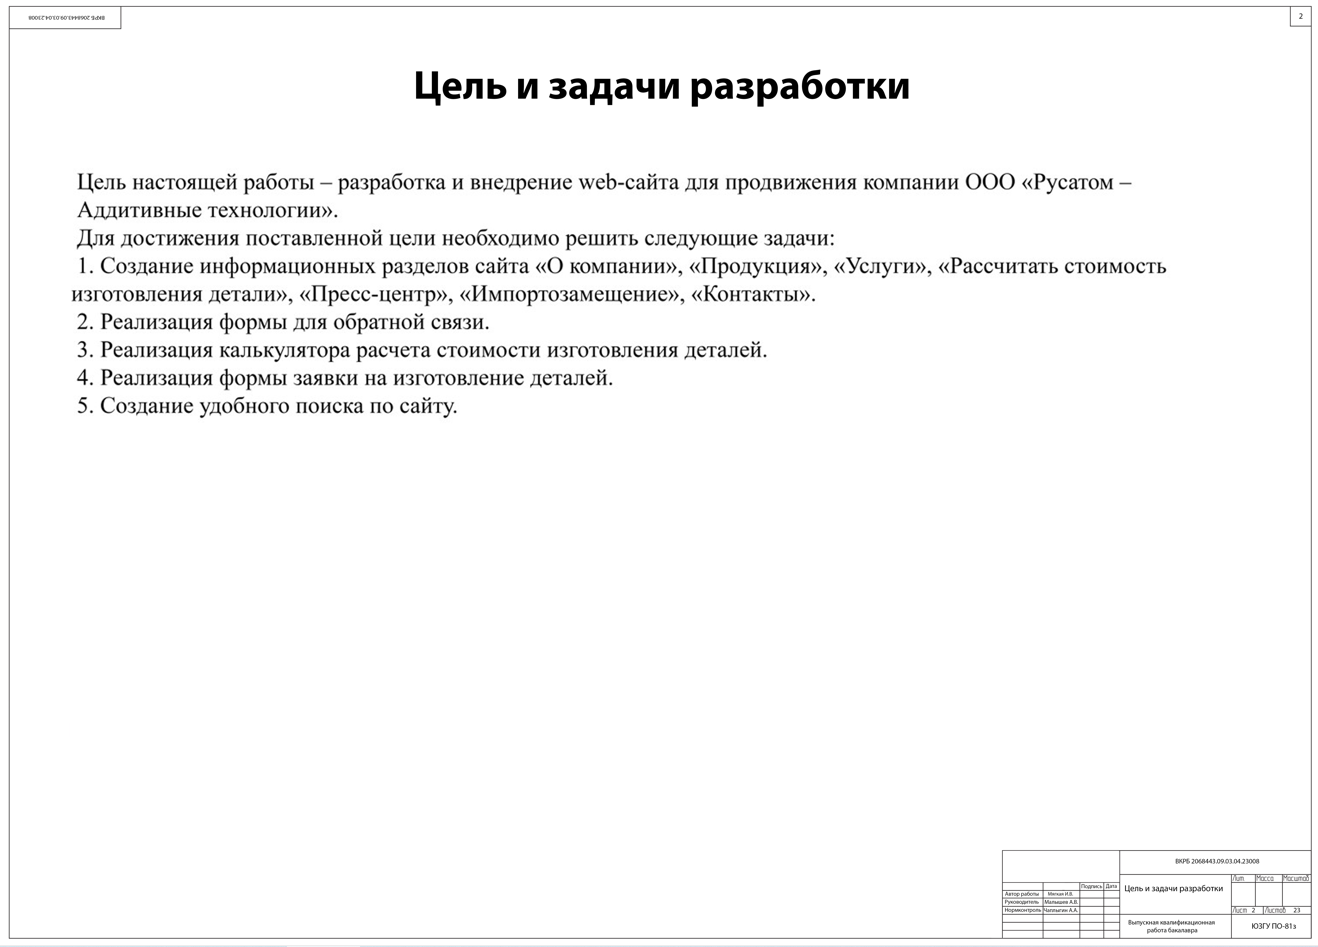
\includegraphics[width=0.82\linewidth]{плакат2.png}
    \заголовок{Цель и задачи разработки}
    \label{pl2:image}      
\end{плакат}

\begin{плакат}
    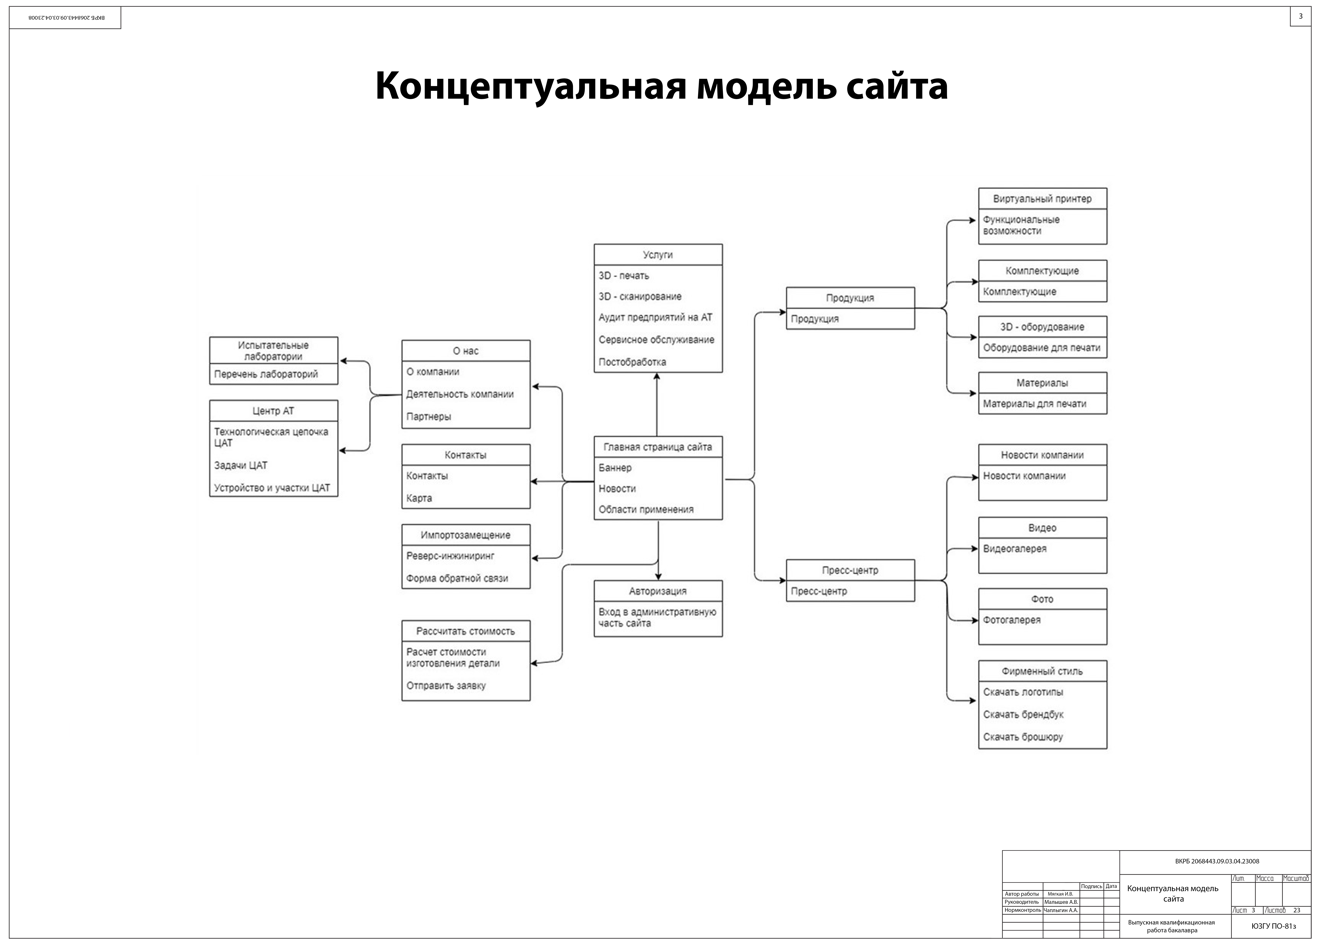
\includegraphics[width=0.82\linewidth]{плакат3.png}
    \заголовок{Концептуальная модель сайта}
    \label{pl3:image}      
\end{плакат}

\begin{плакат}
    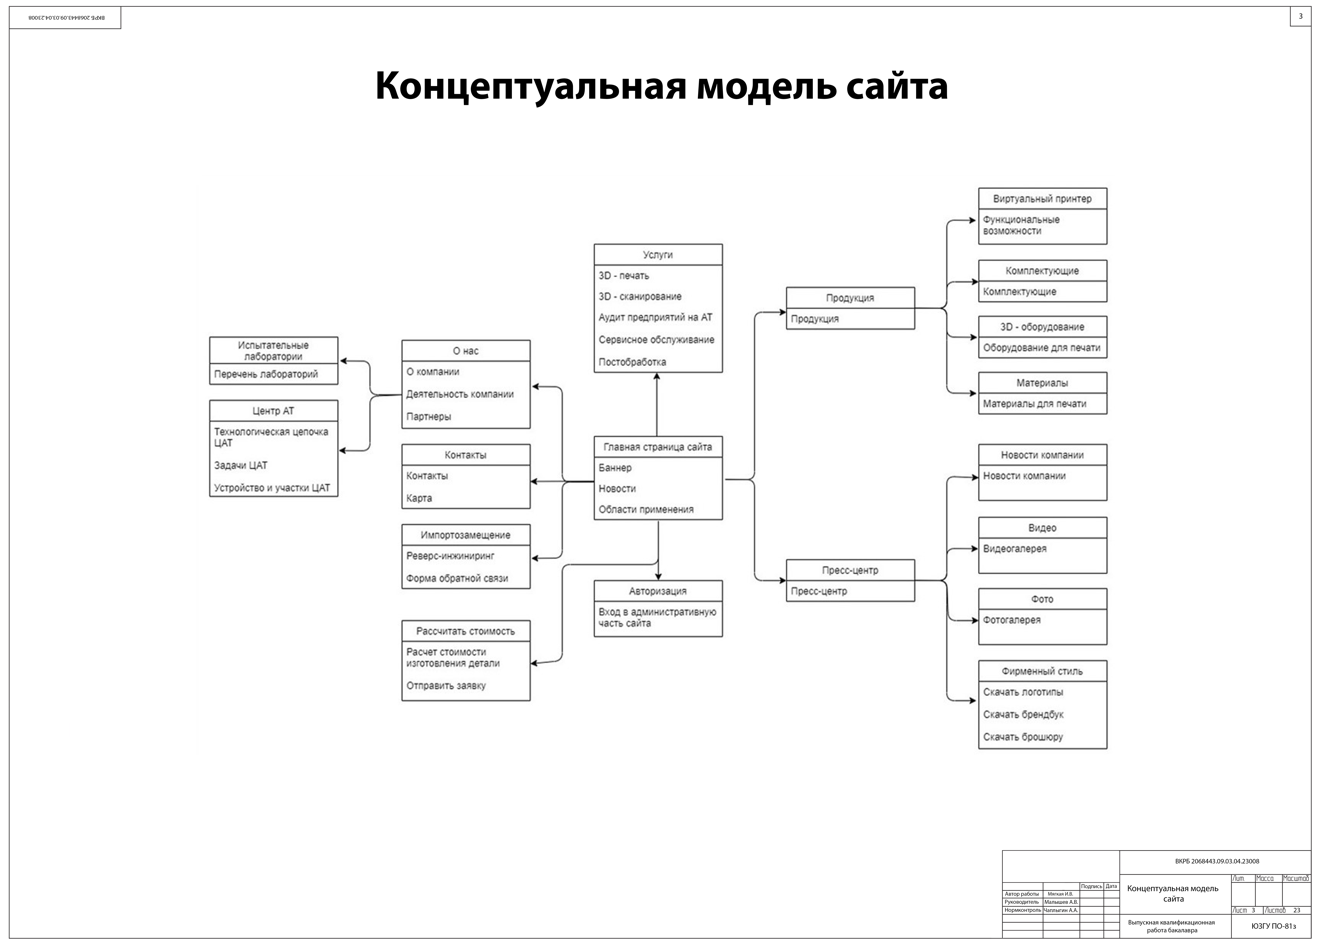
\includegraphics[width=0.82\linewidth]{плакат3.png}
    \заголовок{Еще плакат}
    \label{pl4:image}      
\end{плакат}

\end{landscape}
}\fi
\ifПрактика{}\else{\appendix{Фрагменты исходного кода программы}

main.tex
\lstinputlisting[language=Tex, frame=none]{main.tex}

ТехПроект.tex
\lstinputlisting[language=Tex, frame=none]{ТехПроект.tex}

\ifВКР{
\newpage
\addcontentsline{toc}{section}{На отдельных листах (CD-RW в прикрепленном конверте)}
\begin{center}
\textbf{Место для диска}
\end{center}
}\fi
}\fi
\end{document}
